\chapter{Évaluation}
\label{chap:evaluation}

\todo{}

\section{Évaluation des besoins exprimés par les utilisateurs}

\todo{}

\section{Évaluation de la description}

Le plan de description que nous avons présenté dans le chapitre \ref{chap:implementation} a été utilisé comme référence pour générer les description des carrefours. Cette description, bien qu'issue d'échanges avec des personne concernées ne répond pas nécessairement à la diversité des besoins exprimés par les utilisateurs. Pour évaluer sa correspondance avec les usages, et déterminer quels éléments pourraient être modularisés, nous avons réalisé une enquête auprès de professionnels liés à la déficience visuelle.

\newpar{}

L'enquête a été réalisée avec l'outil en ligne LimeSurvey. Elle présente aux utilisateurs deux descriptions de carrefours générées par la chaîne présentée en partie \ref{sec:implementation_segmentation}. Les deux carrefours choisis et leurs descriptions associées sont illustrés en figure \ref{fig:evaluation_carrefours_enquete}.

\newpar{}

\begin{figure}[ht]
    \centering
    \begin{subfigure}[t]{.49\linewidth}
        \centering
        
\includegraphics[width=\textwidth]{images/placeholder.jpg}
        \caption{Le premier carrefour, en croix, présente des traversées complexes et longues pouvant passer par plusieurs îlots.}
        \label{fig:evaluation_carrefour_master}
    \end{subfigure}
    \begin{subfigure}[t]{.49\linewidth}
        \centering
        
\includegraphics[width=\textwidth]{images/placeholder.jpg}
        \caption{Le second carrefour, à 5 branches, présente des branches moins orthogonales et des difficultés sur le trottoir comme une sortie de garage au sud-ouest.}
        \label{fig:evaluation_carrefour_manon}
    \end{subfigure}
    \caption{Les deux carrefours de Clermont-Ferrand choisis pour l'enquête présentent deux configurations différentes. Il s'agit dans les deux cas de carrefours complexes présentant des îlots et des particularités dans leurs cheminements.}
    \label{fig:evaluation_carrefours_enquete}
\end{figure}

Pour chaque carrefour, l'enquête présente une orthophotographie Google Satellite interactive centrée sur le carrefour et une vue immersive Google StreetView au même emplacement pour permettre aux participants de se familiariser avec le carrefour. Elle présente enfin la description du carrefour telle que générée par la chaîne présentée en partie \ref{sec:implementation_segmentation}, et invite les participants à modifier cette description pour l'adapter à leurs besoins et leurs pratiques.

\newpar{}

L'enquête a été émise le XX/XX/2023 et les résultats ont été exportés le XX/XX/2023. Nous avons reçu dix réponses.

\todo{}

\section{Évaluation des implémentations}

\label{sec:evaluation_implementation}

Dans le chapitre \ref{chap:implementation}, nous avons présenté les implémentations des méthodes de segmentation et de description de carrefours du chapitre \ref{chap:modelisation}. Ces deux outils, crseg et crmodel, sont évalués dans cette partie pour mesurer leur efficacité et leur précision.

\newpar{}

Nous avons développé un outil d'évaluation aléatoire qui nous permet de comparer les résultats de notre algorithme avec l'œil d'un expert. L'outil permet à l'utilisateur de charger le résultat calculé sur une zone d'intérêt fixe, et propose ensuite d'évaluer dans un ordre aléatoire les carrefours traités. L'interface d'évaluation (Figure~\ref{fig:evaluationTool}) est composée de deux panneaux : à gauche, un formulaire simple permet à l'utilisateur d'indiquer en quelques clics les défauts éventuels du résultat, et à droite le carrefour est représenté par un ensemble de polylignes dont les couleurs correspondent au carrefour lui-même et aux différentes branches de ce carrefour. L'ensemble est dessiné sur une orthophotographie, et une série de boutons peut être utilisée à la demande pour afficher le carrefour dans les outils web habituels (\gls{osm}, Google Maps, Google Street View).

\begin{figure}[ht]
    \centering
    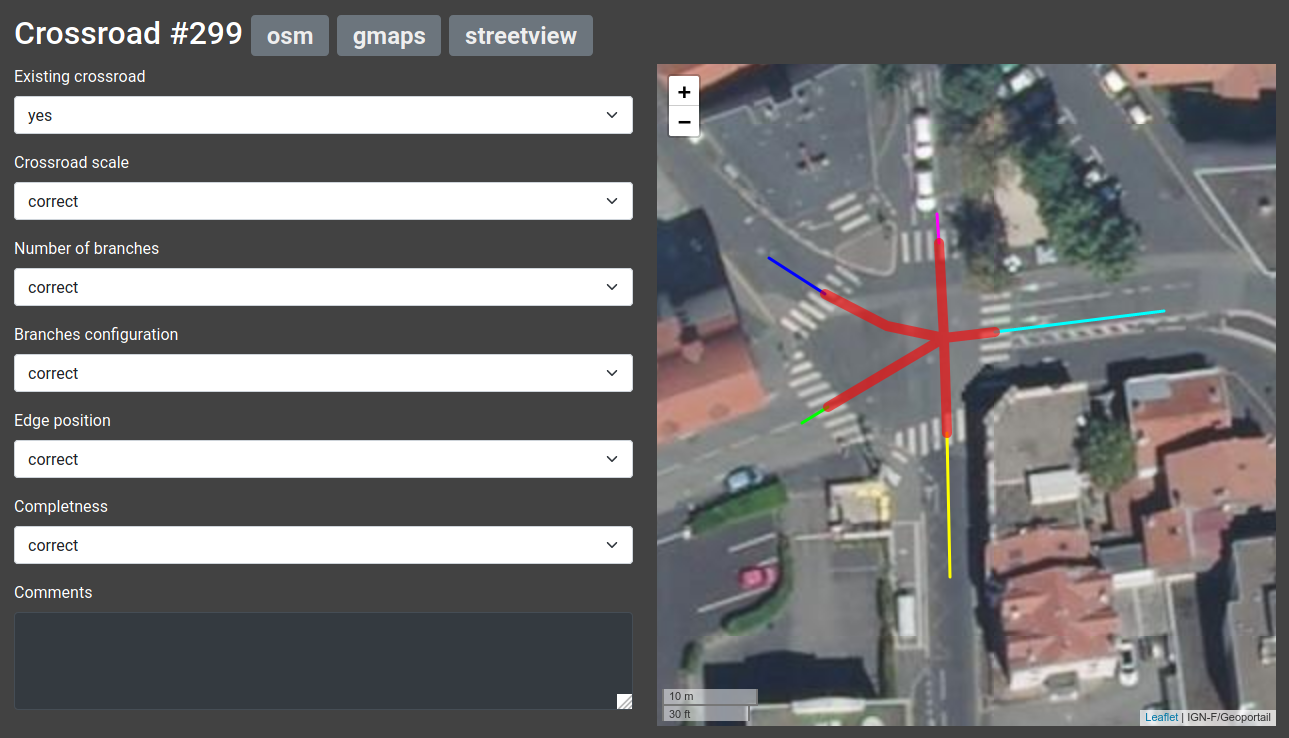
\includegraphics[width=0.8\textwidth]{images/evaluation/evaluation-xxx.png}
    \caption{Interface de l'outil d'évaluation. Source: \cite{Favreau2022}.}
    \label{fig:evaluationTool}
\end{figure}

\newpar{}

L'outil génère un fichier d'évaluation pour chaque zone d'intérêt, qui peut être exploré à l'aide d'une interface dédiée (Figure~\ref{fig:explorer}), afin d'avoir un aperçu synthétique du résultat de l'algorithme dans la zone considérée.

\begin{figure}[ht]
    \centering
    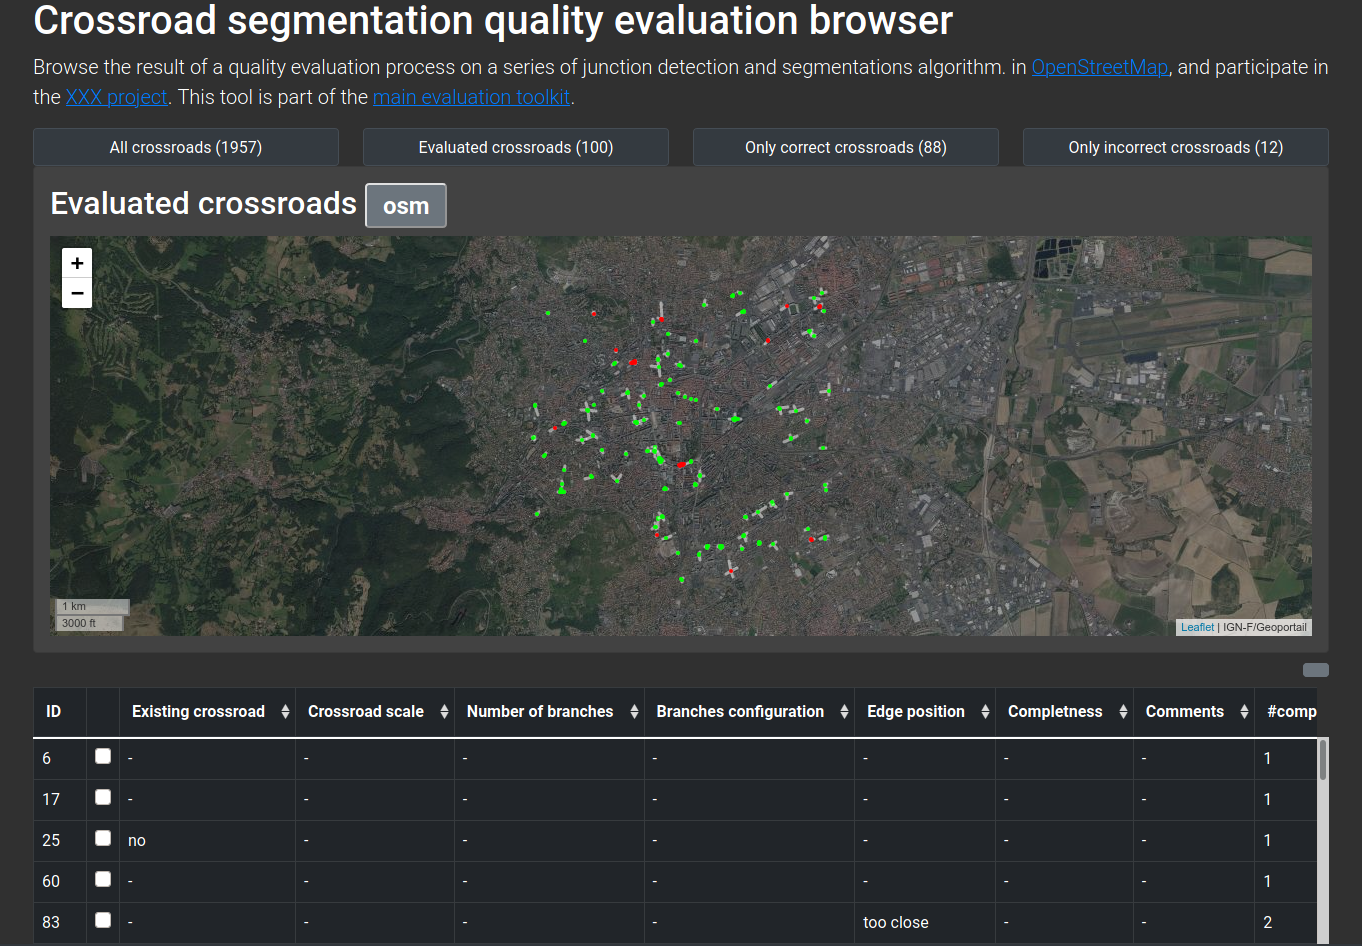
\includegraphics[width=0.8\textwidth]{images/evaluation/eval-browser-xxx.png}
    \caption{Interface pour explorer les évaluations réalisées. Source: \cite{Favreau2022}.}
    \label{fig:explorer}
\end{figure}

\subsection{Évaluation de crseg}

Pour l'évaluation statistique, nous avons sélectionné trois villes de taille représentative des villes françaises : la ville 1 (Paris, 10 785 092 habitants dans l'aire urbaine), la ville 2 (Nantes, 650 081 habitants dans l'aire urbaine) et la ville 3 (Clermont-Ferrand, 268 696 habitants dans l'aire urbaine). Sur chacune d'entre elles, nous avons sélectionné un point et récupéré toutes les données \gls{osm} dans un rayon de deux kilomètres autour de ce point (voir Figure~\ref{fig:regions}).

\newpar{}

\begin{figure}[ht]
    \centering
    \begin{subfigure}[t]{0.49\linewidth}
        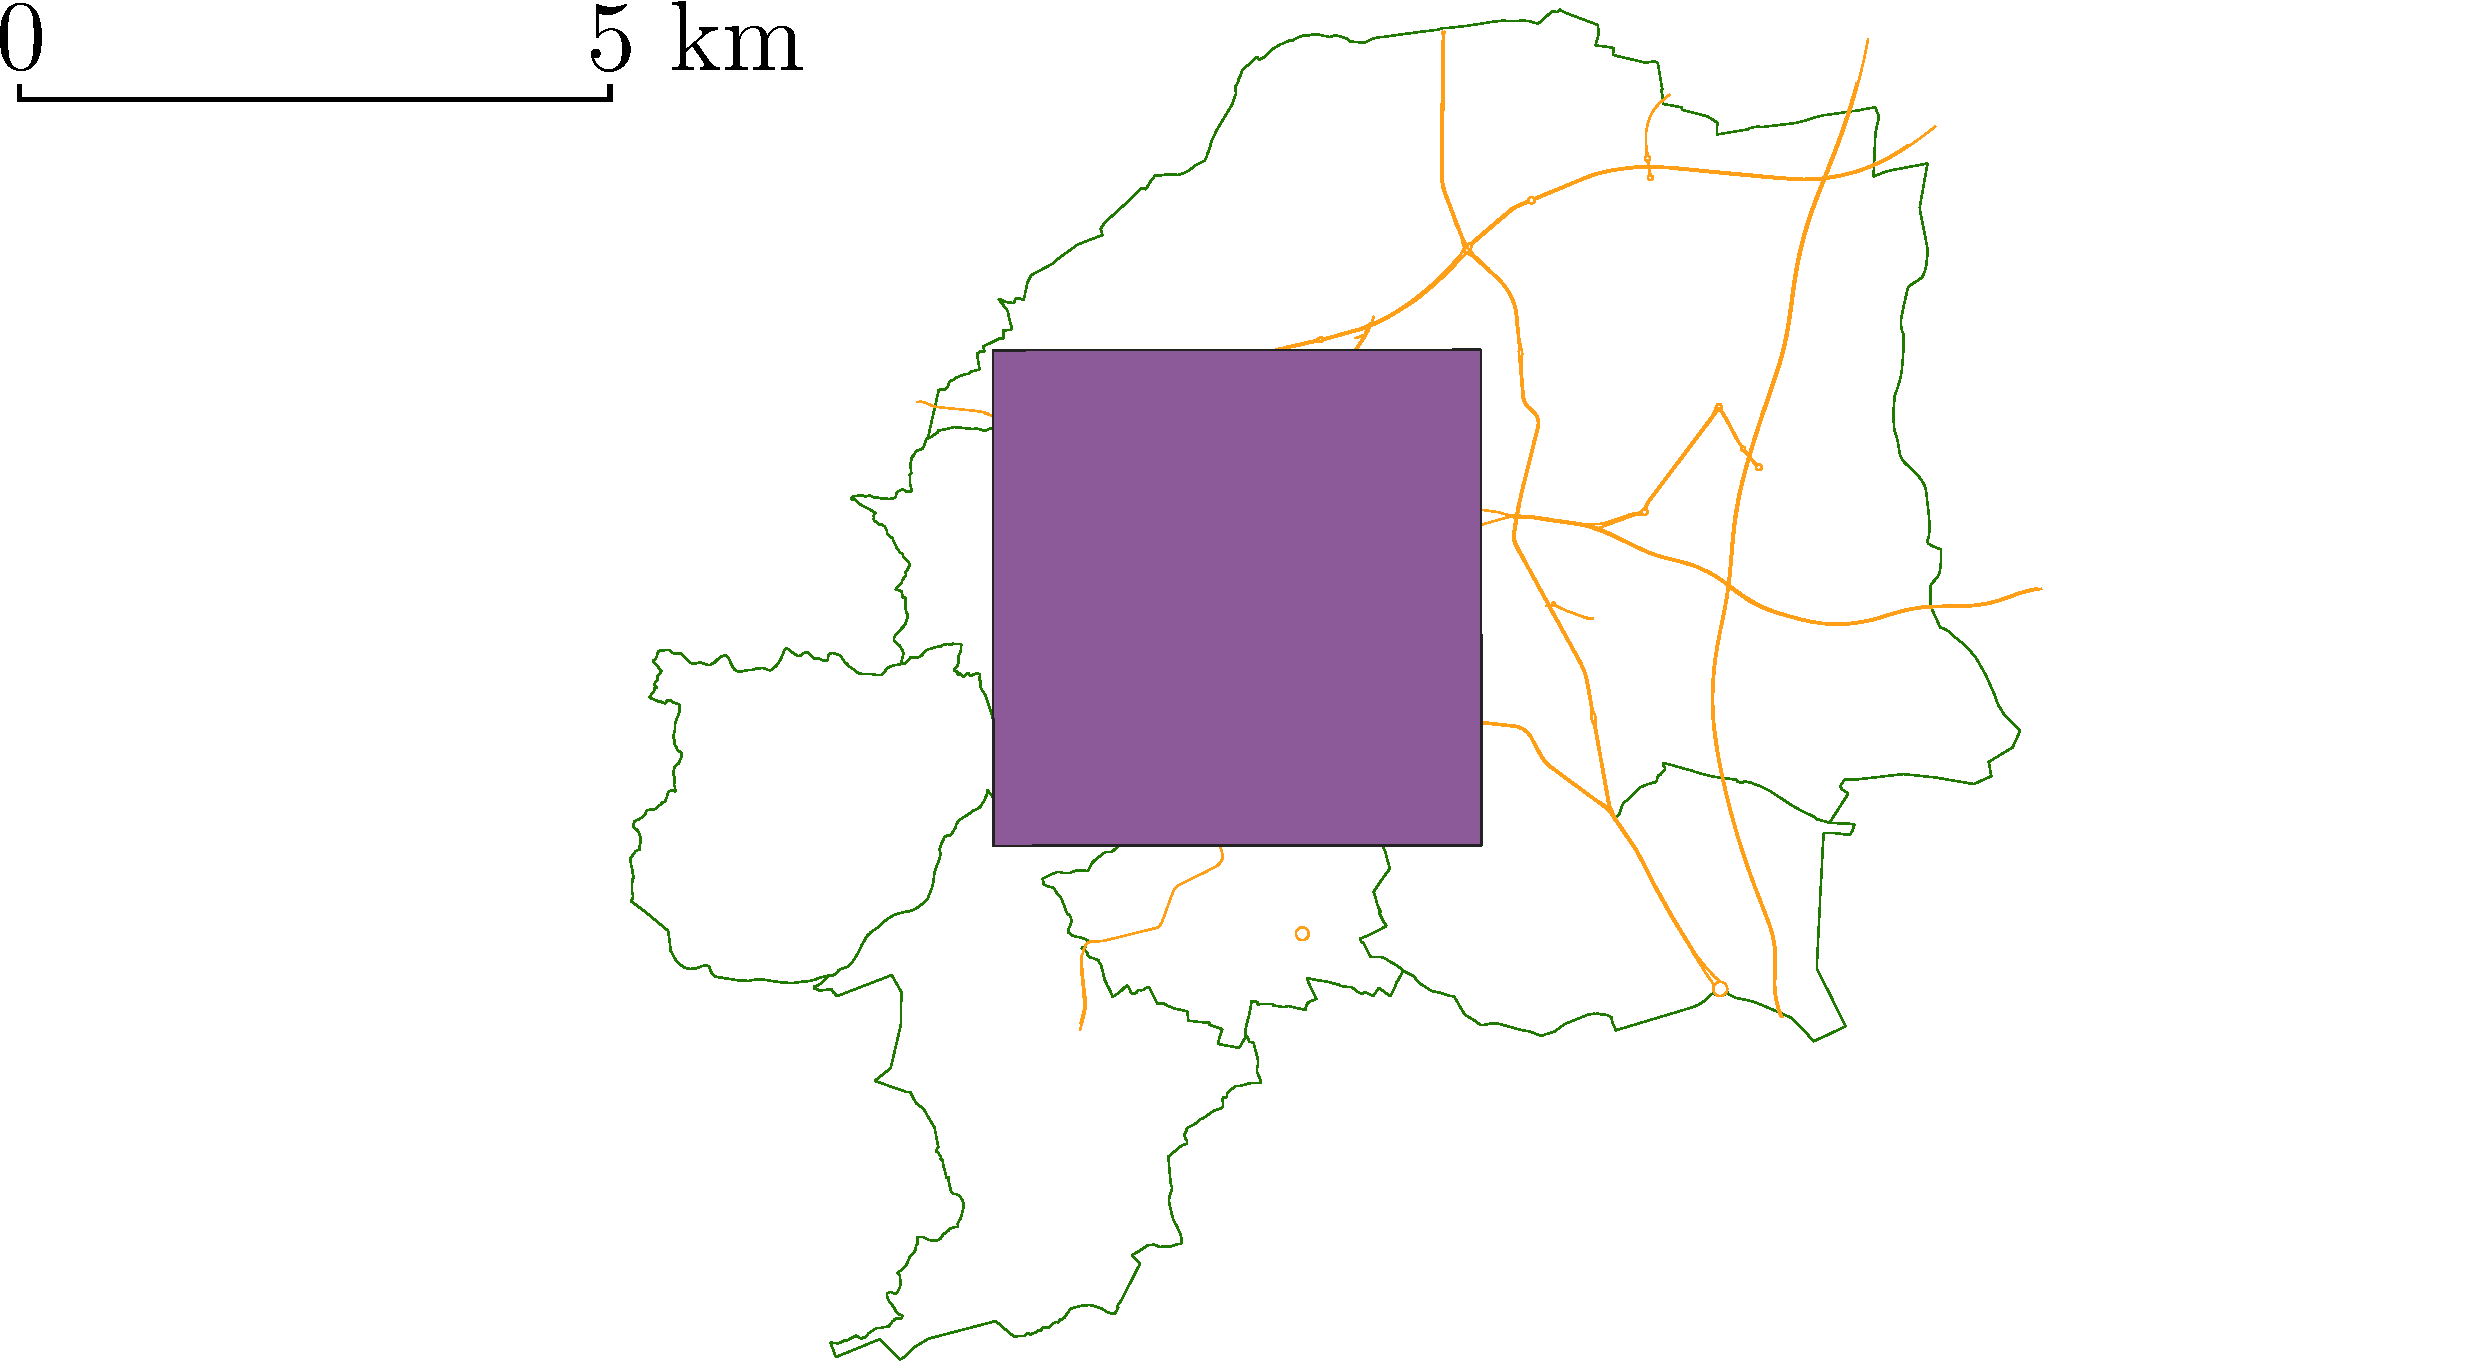
\includegraphics[width=\textwidth]{images/evaluation/crseg/clermont.pdf}
        \caption{Région sélectionnée centrée sur le centre historique de Clermont-Ferrand. La région contient des rues qui font partie des villes suivantes : Clermont-Ferrand, Aubière, Beaumont, Ceyrat, Royat et Chamalières.\label{fig:clermontRegion}}
    \end{subfigure}
    \begin{subfigure}[t]{0.49\linewidth}
        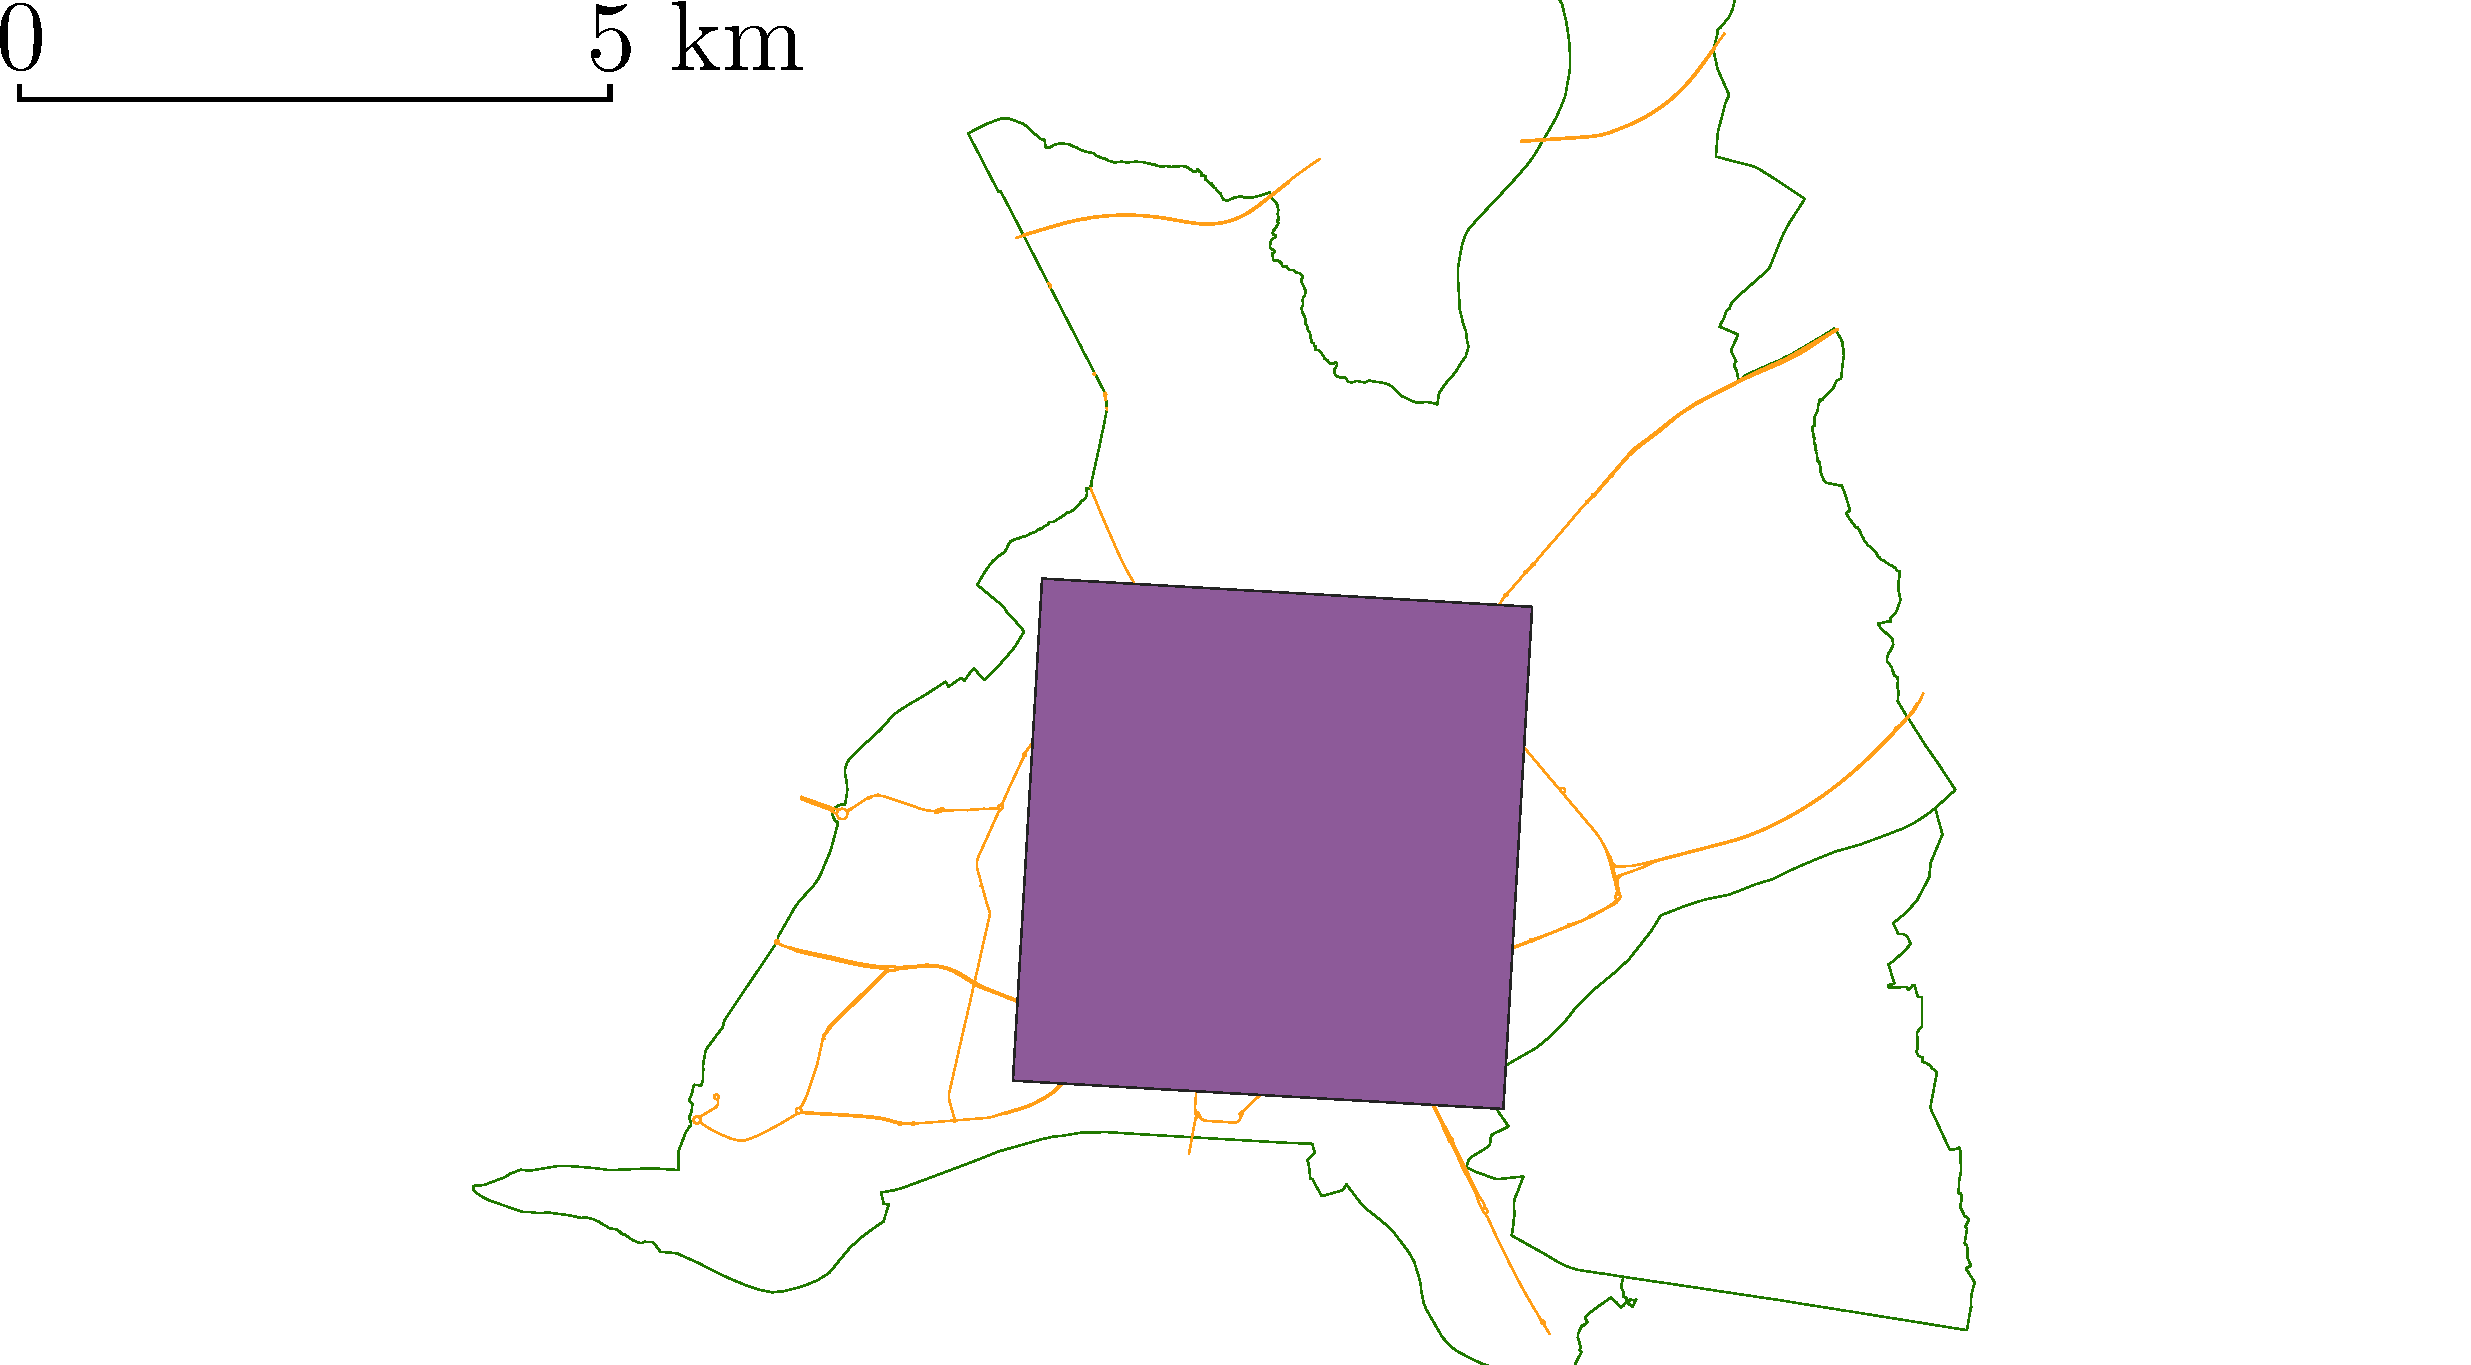
\includegraphics[width=\textwidth]{images/evaluation/crseg/nantes.pdf}
        \caption{Région sélectionnée centrée sur le centre historique de Nantes. La région contient également des rues qui font partie de Saint-Sébastien sur Loire.\label{fig:nantesRegion}}
    \end{subfigure}
    \begin{subfigure}[t]{0.49\linewidth}
        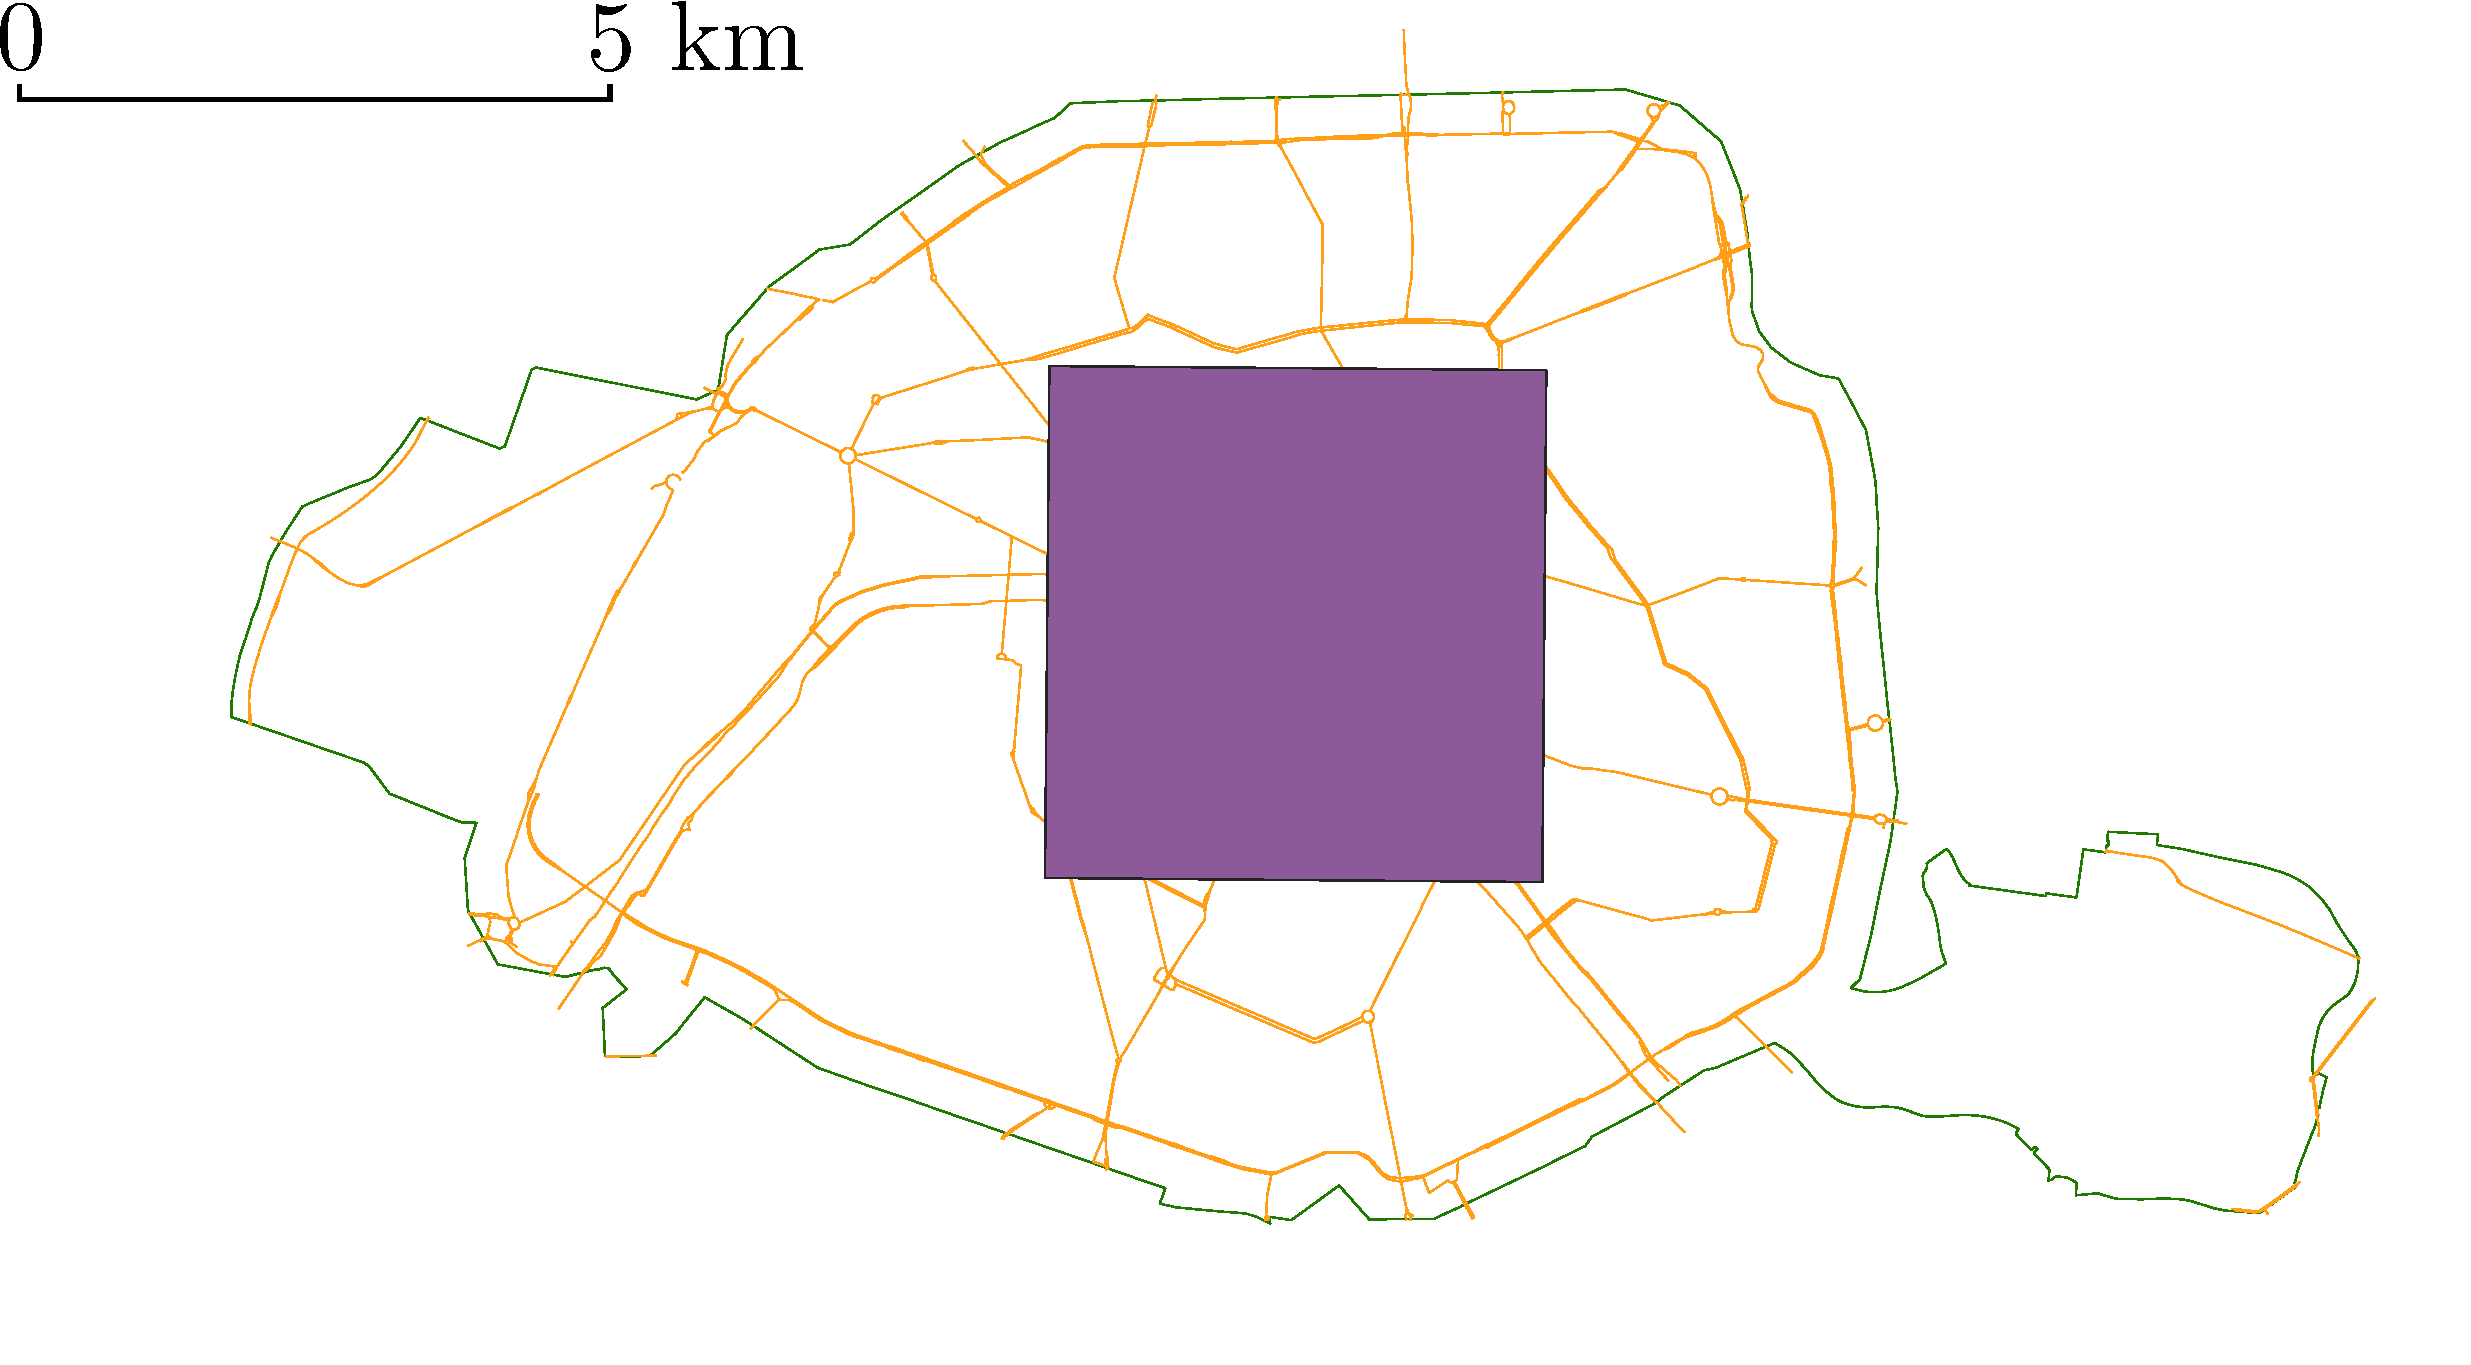
\includegraphics[width=\textwidth]{images/evaluation/crseg/paris.pdf}
        \caption{Région sélectionnée centrée sur Paris.\label{fig:parisRegion}}
    \end{subfigure}
    \caption{Régions sélectionnées pour l'évaluation statistique. Source: \cite{Favreau2022}.}
    \label{fig:regions}
\end{figure}

Nous avons appliqué le processus de segmentation sur chacune des régions, obtenant un total de 5 553 carrefours. Le tableau~\ref{tab:initRegions} donne pour chaque région la répartition des carrefours selon leur complexité : carrefours avec un seul noeud, carrefours avec plusieurs noeuds dont un seul a une cardinalité supérieure à 2, carrefours avec plusieurs noeuds de cardinalité supérieure à 2.

\newpar{}

\begin{table}[ht] 
    \centering
    \footnotesize
    \begin{tabular}{c|c|c|c|c}
    Région & \#total & \#simple &\#intermédiaire & \#complexe \\
    \hline
     1 & 1,818 & 265 & 1,541  & 12 \\
     2 & 1,778 & 573 & 1,190 & 15 \\
     3 & 1,957 & 1,006 & 931  & 20 \\
     \hline
     toutes & 5,553  & 1,844 & 3,662 &	47  \\
     \hline
     ratio & & 33.2\% & 65.9\% & 0.8\% \\
    \end{tabular}
    \caption{Complexité des carrefours générés dans chaque région : carrefours avec un seul nœud, carrefours avec plusieurs nœuds dont un seul a une cardinalité supérieure à 2, carrefours avec plusieurs nœuds de cardinalité supérieure à 2. Source: \cite{Favreau2022}.}
    \label{tab:initRegions}
\end{table}

\begin{table}[ht]
    \centering
    \footnotesize
    \begin{tabular}{c|c|c|c|c}
    Région & \#total & \#simple &\#intermédiaire& \#complexe \\
    \hline
     1 & 100 & 29 & 70 & 1 \\
     2 & 100 & 17 & 83 & 0 \\
     3 & 100 & 52 & 45 & 3 \\
     \hline
     toutes & 300 & 98 & 198 & 4 \\
     \hline
     ratio & &  32.7\% & 66\% & 1.3\%\\
    \end{tabular}
    \caption{Complexité des carrefours choisis au hasard : carrefours avec un seul nœud, carrefours avec plusieurs nœuds dont un seul a une cardinalité supérieure à 2, carrefours avec plusieurs nœuds de cardinalité supérieure à 2. Source: \cite{Favreau2022}.}
    \label{tab:selectedRegions}
\end{table}

Nous avons utilisé l'outil d'évaluation présenté dans la partie \ref{sec:evaluation_implementation}
dans chaque région, en évaluant au hasard 100 carrefours dans chaque région. Le tableau~\ref{tab:selectedRegions} montre que la répartition des carrefours en fonction de leur complexité est comparable à celle de toutes les régions. L'évaluation nécessitait de répondre aux questions suivantes:
\begin{itemize}
    \item Carrefour existant: \textit{oui} ou \textit{non},
    \item Échelle du carrefour: \textit{correcte}, \textit{trop grande} ou \textit{trop petite},
    \item Nombre de branches: \textit{correct}, \textit{trop peu} ou \textit{trop nombreuses},
    \item Configuration des branches: \textit{correcte}, \textit{deux branches ou plus sont fusionnées}, \textit{une branche ou plus sont divisées} ou \textit{branches fusionnées et divisées},
    \item Position des bordures (relatif au centre du carrefour): \textit{correctes}, \textit{trop proches} ou \textit{trop éloignées},
    \item Complétude: \textit{correcte}, \textit{parties manquantes} ou \textit{parties en trop}.
\end{itemize}

\newpar{}

Sur ces 300 carrefours, 245 ont été évalués comme valides en comparant la segmentation avec l'orthophotographie proposée par l'interface (voir Tableau~\ref{tab:nbRegions}).

\newpar{}

\begin{table}[ht]    
    \centering
    \footnotesize
    \begin{tabular}{c|c|c|c}
         Région & \#total & \#sélectionné & \#segmentation valide \\
         \hline
         1 & 1,818 & 100 & 81 \\
         2 & 1,778 & 100 & 76 \\
         3 & 1,957 & 100 & 88 \\
    \end{tabular}
    \caption{Description du jeu de données : pour chaque région, le nombre de carrefours obtenus par notre algorithme, le nombre de carrefours sélectionnés aléatoirement (100), et le nombre de segmentations valides par rapport à l'orthophotographie. Source: \cite{Favreau2022}.}
    \label{tab:nbRegions}
\end{table}


Sur les 55 carrefours restants, 26 sont affectés par un problème d'ajustement des limites, l'orthophotographie montrant un passage piéton qui aurait dû être inclus dans la segmentation.
Après analyse, 11 carrefours sont concernés par des passages piétons manquants dans \gls{osm}, 3 carrefours par un passage piétons dépassé ou mal positionné, et 2 carrefours car une rue adjacente est une rue piétonne selon \gls{osm}, ce qui semble incorrect au regard de l'orthophotographie. Les 10 autres limites mal positionnées nécessiteraient un ajustement local du paramètre C0.

\newpar{}

Parmi les carrefours restants, 21 ont été considérés comme ayant des parties manquantes ou comme étant à une échelle trop grande ou trop petite. Il y a plusieurs causes à cela : 
\begin{itemize}
    \item pour 2 d'entre eux, il s'agit d'une voie manquante dans la modélisation \gls{osm}, 
    \item pour 3 autres, une rue adjacente a été identifiée dans \gls{osm} comme n'étant pas accessible aux voitures, 
    \item pour 4 autres, il s'agit de routes bordant ou entrant dans une place, espaces non pris en compte par l'algorithme,
    \item pour 12 d'entre eux, l'ajustement local du paramètre C1 ou C2 aurait permis de corriger la segmentation.
\end{itemize}

\newpar{}

Deux carrefours ont été considérés comme inexistants. Après analyse, il s'agissait d'approximations dans la modélisation \gls{osm} (voie privée mal étiquetée, modélisation inexacte d'un passage piéton linéaire).

\newpar{}

L’un des carrefours avait ses trois branches combinées en une seule. L'algorithme n'a pas interprété correctement un carrefour en T dans un quartier résidentiel où chaque branche portait le même nom.

\newpar{}

L’un des carrefours a vu l’une de ses branches divisée en deux branches. Après analyse, ces deux voies correspondaient à la desserte d'un parking et n'avaient pas de nom, ce qui empêchait l'algorithme de les associer.

\newpar{}

Enfin, nous avons également identifié un carrefour situé au milieu d'un parc, et 3 carrefours au milieu de parkings, ce qui invite à un travail plus poussé sur le filtrage des données \gls{osm}.

\newpar{}

En résumé (Figure~\ref{fig:camembert}), la segmentation de 23 carrefours peut être corrigée en ajustant localement l'un des trois paramètres de la méthode, 18 carrefours sont imprécis en raison de l'absence ou de l'imprécision des données dans \gls{osm}, et 14 carrefours illustrent le manque de généralité de notre algorithme, qui ne prend pas en compte les voies fermées aux voitures, les voies sans nom, les carrefours ayant le même nom sur toutes les branches, ou encore le contexte (place, parc, parking).

\begin{figure}[ht]
    \centering
    \footnotesize
    \begin{tikzpicture}
        \pie[color = {
        blue!60, 
        blue!45, 
        gray, orange}]{81.6/A, 6/B, 4.6/C, 7.7/D}
    \end{tikzpicture}
    \caption{Répartition des carrefours considérés lors de notre processus d'évaluation (Table~\ref{tab:nbRegions}) en fonction de leur typologie. A (245 carrefours) : segmentation correspondant à l'orthophotographie, B (18 carrefours) : manque ou imprécision dans \gls{osm}, C (14 carrefours) : régions non supportées, D (23 carrefours) : nécessite un ajustement local des paramètres. Source: \cite{Favreau2022}.}
    \label{fig:camembert}
\end{figure}

\subsection{Évaluation de crmodel}

L'évaluation de l'implémentation de crmodel permet d'estimer sa capacité à générer des descriptions satisfaisantes au regard des données disponibles dans OpenStreetMap. Nous avons choisi de réaliser l'évaluation sur trois villes françaises : Lyon (522 969 habitants), Clermont-Ferrand (147 865 habitants) et Brive-la-Gaillarde (46 330 habitants).

\newpar{}

La qualité de la description a été évaluée en fonction de sa conformité avec le terrain et les données disponibles. Une description définie comme correcte correspond au terrain. Une description partiellement correcte indique qu'elle correspond en partie au terrain mais que les données, l'implémentation ou la segmentation étaient insuffisantes pour fournir une description complète. Une description incorrecte ne correspond pas du tout au terrain. Des descriptions de 20 carrefours par ville, choisis au hasard, ont été générées et l'instanciation des branches et des traversées a été évaluée. L'évaluation est basée sur l'outil proposé par en partie \ref{sec:evaluation_implementation}. Les valeurs des attributs OpenStreetMap ont été confrontées aux images aériennes afin d'évaluer les problèmes de données. Les dispositifs sonores des passages piétons n'ont pas été pris en compte car les images aériennes ne permettent pas de vérifier cette information. L'évaluation nécessitait de répondre aux questions suivantes:
\begin{itemize}
    \item Première branche au nord: \textit{oui}, \textit{non} ou \textit{indéfini}
    \item Présence des voies sur OSM: \textit{corrects}, \textit{attributs manquants} ou \textit{objets manquants},
    \item Nombre de voies: \textit{correct}, \textit{trop peu} ou \textit{trop nombreuses},
    \item Types de voies: \textit{corrects}, \textit{incorrects},
    \item Ordre des voies: \textit{corrects}, \textit{incorrects},
    \item Présence des passages piétons sur OSM: \textit{corrects}, \textit{attributs manquants} ou \textit{objets manquants},
    \item Génération des traversées: \textit{correctes}, \textit{incorrectes} ou \textit{trop peu} ou \textit{trop nombreuses}
\end{itemize}

\begin{figure}[ht]
    \centering
    \begin{tikzpicture}
        \pie[color = {
        blue!60, 
        blue!45, 
        gray}]{53.7/A, 14.8/B, 31.5/C}
    \end{tikzpicture}
    \caption{Distribution des types de problèmes rencontrés au cours du processus d'évaluation. A (29 carrefours) : objets ou attributs manquants dans OpenStreetMap, B (8 carrefours) : problèmes d'implémentation, soit des attributs non supportés, soit des erreurs d'algorithme, C (17 carrefours) : erreurs mélangeant l'implémentation, la segmentation et les problèmes de données.}
    \label{fig:camissues}
\end{figure}

\newpar{}

La description du nombre et des noms des branches est celle qui donne les meilleurs résultats. Ceux-ci dépendent principalement de la qualité de la segmentation (19 intersections sur 20, soit 95\% des erreurs rencontrées). Les descriptions des voies des branches et les descriptions des traversée sont plus sensibles à la qualité des données OpenStreetMap (respectivement 26 sur 41 et 30 sur 36 intersections, soit 63,4\% et 83,3\% des erreurs rencontrées). Les voies sont également fortement affectées par les erreurs d'implémentation (19 intersections sur 41, soit 46,3\% des erreurs rencontrées) car toutes les clés \gls{osm}, notamment celles relatives aux lignes de bus, n'ont pas été prises en compte.  Ces résultats sont résumés dans le tableau~\ref{tab:descqualitybydesctype}.

\begin{table}[ht]
    \begin{center}
        \footnotesize
        \begin{tabular}{ c | c | c | c }
            Qualité de la description & Nombre et noms des branches & Voies des branches & Traversées\\
            \hline
            Correct & 40  & 19 & 24 \\
            Partiellement correct & 17 & 40 & 34 \\
            Incorrect & 3 & 1 & 2 \\
            \hline
            Nombre de carrefours & 60 & 60 & 60
        \end{tabular}
        \caption{Qualité de la description par type de données.}
        \label{tab:descqualitybydesctype}
    \end{center}
\end{table}

\newpar{}

Les résultats globaux indiquent que seuls 6 carrefours de l'échantillon ont été parfaitement décrits. D'autre part, 56 intersections ont été au moins partiellement décrites correctement. Le principal problème à l'origine de la dégradation de la description est la qualité des données \gls{osm} (Figure~\ref{fig:camissues}) où les clés ou les objets manquants ont eu un impact sur la description. On peut cependant noter que les trois villes choisies n'ont pas la même qualité de données \gls{osm} (Tableau~\ref{tab:osmqualityissues}).

\begin{table}[ht]
    \begin{center}
        \footnotesize
        \begin{tabular}{c | c | c | c }
            Type de problème & Lyon & Clermont-Ferrand & Brive-la-Gaillarde\\
            \hline
            Lié à \gls{osm} & 8  & 13 & 17 \\
            Non-lié à \gls{osm} & 9 & 4 & 3 \\
            \hline
            Nombre de problèmes & 17 & 17 & 20 \\
            Nombre de carrefours & 20 & 20 & 20
        \end{tabular}
        \caption{Problèmes rencontrés et leur relation avec les données \gls{osm} par ville.}
        \label{tab:osmqualityissues}
    \end{center}
\end{table}

\section{Évaluation du pipeline de conception de description}

\todo{}